\documentclass[11pt]{article}

\usepackage{times}
\usepackage[utf8]{inputenc}
\usepackage[T1]{fontenc}
\usepackage{url}
\usepackage{graphics}
\usepackage{graphicx}
\usepackage{color}
\usepackage{amsfonts}
\usepackage{amsmath}
\usepackage{amssymb}
\usepackage{booktabs}
\usepackage{multirow}
\usepackage{tabularx}
\usepackage{longtable}
\usepackage{subcaption}
\usepackage{caption}
\captionsetup{font=small,labelfont=bf}
\captionsetup[subfigure]{font=footnotesize,labelfont=normalfont}
\captionsetup{skip=4pt}
\usepackage{algorithm}
\usepackage{algpseudocode}
\usepackage{geometry}
\usepackage{pdflscape}
\usepackage{tikz}
\usetikzlibrary{positioning,fit,arrows.meta}
\usepackage{fancyhdr}
\usepackage{hyperref}
\usepackage{xcolor}

% Geometry setup
\geometry{left=2.8cm,right=2.8cm,top=2.4cm,bottom=2.4cm,headheight=14pt}
% Overleaf-friendly: all figures in ./figures/
\graphicspath{{./figures/}}
\pagestyle{fancy}
\lhead{RL Hockey Project}
\chead{}
\rhead{\thepage}
\cfoot{}
\setlength{\textfloatsep}{8pt plus 2pt minus 2pt}
\setlength{\floatsep}{6pt plus 2pt minus 2pt}
\setlength{\intextsep}{8pt plus 2pt minus 2pt}
\setlength{\abovedisplayskip}{6pt}
\setlength{\belowdisplayskip}{6pt}

\title{World-Model Based Reinforcement Learning for Hockey:\\
        DreamerV3 with Adaptive Opponent Curriculum}
\author{Carl Kueschall\\
        University of T\"ubingen}
\date{Winter Semester 2025/26}

\begin{document}

\maketitle

% ============================================================================
% SECTION 1: INTRODUCTION
% ============================================================================
\section{Introduction}\label{sec:intro}

\textit{Note: Originally a two-person project; co-author exmatriculated. Work completed by remaining author.}

\medskip
The hockey environment~\cite{martius2024} presents a challenging continuous control problem in an adversarial setting. Two agents compete in an air-hockey game with 18-dimensional state observations encoding positions, velocities, and puck state, while each player controls 4 continuous action dimensions. Episodes last up to 250 timesteps with extremely sparse rewards: $+10$ for scoring, $-10$ for conceding, and $0$ otherwise. This sparsity makes credit assignment difficult---agents must learn complex behaviors (positioning, puck control, shooting, defending) from reward signals that occur only at episode boundaries.

I implement DreamerV3~\cite{hafner2024}, which learns a world model from real rollouts and trains the policy in imagined latent trajectories. Starting from NaturalDreamer\footnote{\url{https://github.com/InexperiencedMe/NaturalDreamer}}, I add hockey-specific components: Two-Hot Symlog heads, DreamSmooth~\cite{dreamsmooth2023}, sparse-event loss weighting, PFSP self-play~\cite{vinyals2019}, and an adaptive opponent curriculum. The main practical result is that late gains are driven more by recursive pool curation than by further fixed-bot training.


% ============================================================================
% SECTION 2: METHODS
% ============================================================================
\section{Methods}\label{sec:method}

\subsection{DreamerV3: World-Model Based RL}\label{subsec:dreamer-method}

\subsubsection{World Model Architecture}

DreamerV3~\cite{hafner2024} uses an RSSM with deterministic and stochastic dynamics. The latent state is $s_t=(h_t,z_t)$ with GRU memory $h_t \in \mathbb{R}^{256}$ and categorical $z_t$ (16 variables, 16 classes each). Dynamics: $h_t=\text{GRU}(h_{t-1},z_{t-1},a_{t-1})$; prior $\hat z_t \sim p_\theta(z_t|h_t)$; posterior $z_t \sim q_\phi(z_t|h_t,\text{Enc}(o_t))$. Training uses KL with free nats, plus a continuation head for non-terminal prediction and imagination-time return weighting (Figure~\ref{fig:world_model}).

\begin{figure}[htbp]
\centering
\resizebox{0.98\linewidth}{!}{%
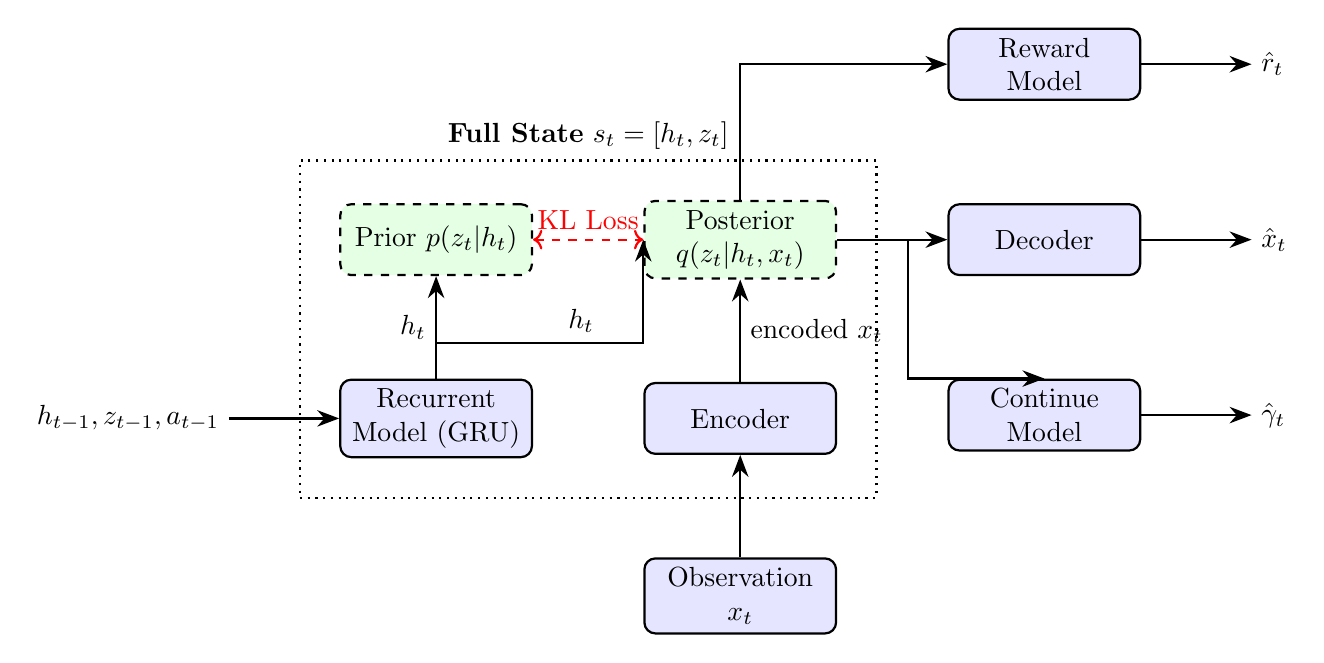
\begin{tikzpicture}[
    node distance=1.3cm and 1.4cm,
    block/.style={rectangle, draw, thick, fill=blue!10, text width=2.2cm, align=center, rounded corners, minimum height=0.9cm},
    latent/.style={rectangle, draw, thick, fill=green!10, text width=2.2cm, align=center, rounded corners, minimum height=0.9cm, dashed},
    arrow/.style={-{Stealth[scale=1.2]}, thick}
]

% Nodes
\node[block] (obs) {Observation $x_t$};
\node[block, above=of obs] (encoder) {Encoder};
\node[block, left=of encoder] (rnn) {Recurrent Model (GRU)};
\node[latent, above=of encoder] (posterior) {Posterior $q(z_t | h_t, x_t)$};
\node[latent, above=of rnn] (prior) {Prior $p(z_t | h_t)$};

\node[block, right=of posterior] (decoder) {Decoder};
\node[block, above=of decoder] (reward) {Reward Model};
\node[block, below=of decoder] (continue) {Continue Model};

% State inputs
\node[left=of rnn] (prevstate) {$h_{t-1}, z_{t-1}, a_{t-1}$};

% Arrows
\draw[arrow] (obs) -- (encoder);
\draw[arrow] (prevstate) -- (rnn);
\draw[arrow] (rnn) -- node[left] {$h_t$} (prior);
% Route above encoder to avoid line crossing the node label
\draw[arrow] (rnn.north) -- ++(0,0.45) -| node[pos=0.35, above] {$h_t$} (posterior.west);
\draw[arrow] (encoder) -- node[right] {encoded $x_t$} (posterior);

% KL Divergence line
\draw[<->, thick, red, dashed] (prior) -- node[above] {KL Loss} (posterior);

% Full state grouping
\node[draw, thick, dotted, fit=(rnn) (posterior), inner sep=0.5cm, label=above:{\textbf{Full State} $s_t = [h_t, z_t]$}] (fullstate) {};

% Outputs
\draw[arrow] (posterior) -- (decoder);
\draw[arrow] (posterior) |- (reward);
% Route around the encoder row to avoid visual strike-through
\draw[arrow] (posterior.east) -- ++(0.9,0) |- (continue.north);

\node[right=of decoder] (recon) {$\hat{x}_t$};
\node[right=of reward] (rew) {$\hat{r}_t$};
\node[right=of continue] (cont) {$\hat{\gamma}_t$};

\draw[arrow] (decoder) -- (recon);
\draw[arrow] (reward) -- (rew);
\draw[arrow] (continue) -- (cont);

\end{tikzpicture}
}
\caption{DreamerV3 world-model training (reality mode): posterior inference from observations, prior matching via KL, and decoder/reward/continue heads from latent state; adapted from~\cite{hafner2024,naturaldreamer}.}
\label{fig:world_model}
\end{figure}

\subsubsection{Key Modifications for Hockey}

Table~\ref{tab:modifications} summarizes our domain-specific modifications. \textbf{DreamSmooth}~\cite{dreamsmooth2023} propagates goal rewards backward: $\tilde{r}_t = \alpha r_t + (1-\alpha)\tilde{r}_{t+1}$ with $\alpha = 0.5$, addressing temporal credit assignment for goals at episode boundaries. In addition, I use inverse-frequency weighting for sparse reward events ($|r|>1$) in reward-head training, capped for stability, to prevent rare goal transitions from being gradient-diluted by the dominant near-zero reward mass.

\begin{table}[h]
\centering
\small
\begin{tabular}{lp{4.2cm}p{4.8cm}}
\toprule
\textbf{Modification} & \textbf{Problem Addressed} & \textbf{Implementation} \\
\midrule
Two-Hot Symlog & Gaussian reward/value heads underfit sparse multimodal targets & 255 bins in symlog space \\
DreamSmooth & Temporal credit assignment & $\tilde{r}_t = \alpha r_t + (1-\alpha)\tilde{r}_{t+1}$, $\alpha=0.5$ \\
Sparse-event loss weighting & Rare goal events underweighted in reward loss & Inverse-frequency weighting for $|r|>1$, clipped for stability \\
Anchor Opponents & Prevent catastrophic forgetting & 10\% weak + 10\% strong in late phase \\
Self-Play + PFSP~\cite{vinyals2019} & Limited diversity & 48-checkpoint pool, variance-weighted PFSP, periodic insertion \\
\bottomrule
\end{tabular}
\caption{Key modifications from baseline DreamerV3 for the hockey domain.}
\label{tab:modifications}
\end{table}

\subsubsection{Recursive Opponent-Pool Management}

The final training policy is controlled by opponent sampling rather than reward shaping, with $\mathbb{P}(\text{anchor})=\rho$ and $\mathbb{P}(\text{self-play})=1-\rho$.
In late runs we set $\rho=0.2$, yielding an empirical distribution close to 80/10/10 (self-play/weak/strong). This keeps fixed-bot competence while maximizing exposure to diverse, hard opponents.
In league runs, PFSP sampling~\cite{vinyals2019} is further blended with a static checkpoint prior from curated league weights, using exponent $\alpha$ (\texttt{self\_play\_prior\_alpha}) so higher-quality checkpoints are sampled earlier without disabling PFSP adaptation.

To avoid selecting brittle checkpoints, I rank candidates with robustness-aware metrics from cross-play:
$\text{RobustScore}=0.60\cdot \text{CP}_{\min}+0.25\cdot \text{Fixed}_{\text{combined}}+0.15\cdot \text{CP}_{\text{mean}}$, and also use $\text{CP}_{q20}$ (20th percentile) for non-transitive settings.

\subsubsection{Behavior Learning}

\textbf{Actor:} Tanh-squashed Gaussian with $\sigma_{\min}=0.1$ plus mean regularization (\texttt{mean\_reg\_scale}) to reduce tanh-saturation drift. \textbf{Critic:} Two-Hot Symlog with slow-critic EMA regularization ($\tau=0.98$). \textbf{Returns:} TD($\lambda$), $\lambda=0.95$, $\gamma=0.997$, with percentile value normalization (5th/95th). \textbf{Actor loss:} $\mathcal{L}_\text{actor}=-\mathbb{E}_{s\sim\text{imagine}}\!\left[\frac{V^\lambda(s)-V(s)}{S}+\eta H[\pi(\cdot|s)]\right]$, fixed $\eta=3\times10^{-4}$.

\begin{figure}[htbp]
\centering
\resizebox{0.92\linewidth}{!}{%
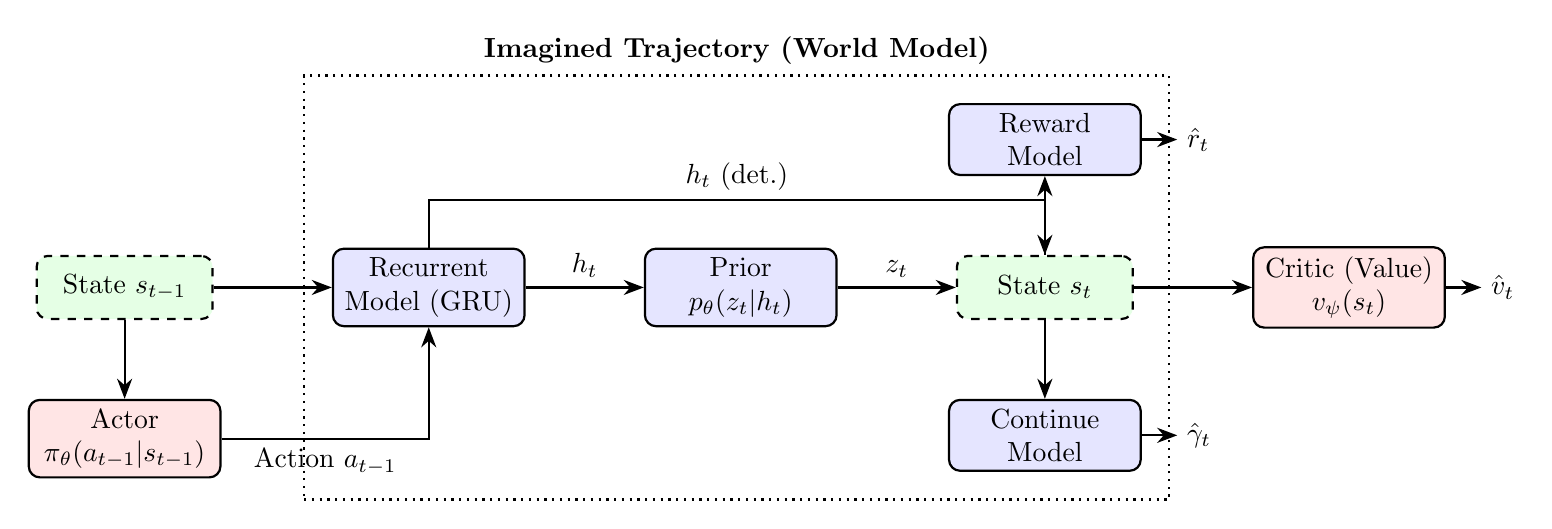
\begin{tikzpicture}[
    node distance=1.4cm and 1.5cm,
    worldmodel/.style={rectangle, draw, thick, fill=blue!10, text width=2.2cm, align=center, rounded corners, minimum height=0.9cm},
    behavior/.style={rectangle, draw, thick, fill=red!10, text width=2.2cm, align=center, rounded corners, minimum height=0.9cm},
    state/.style={rectangle, draw, thick, fill=green!10, text width=2.0cm, align=center, rounded corners, minimum height=0.8cm, dashed},
    arrow/.style={-{Stealth[scale=1.1]}, thick}
]

% Start State
\node[state] (s0) {State $s_{t-1}$};

% Actor (Policy)
\node[behavior, below=1cm of s0] (actor) {Actor\\$\pi_\theta(a_{t-1} | s_{t-1})$};

% RSSM components
\node[worldmodel, right=of s0] (gru) {Recurrent\\Model (GRU)};
\node[worldmodel, right=of gru] (prior) {Prior\\$p_\theta(z_t | h_t)$};

% Next State
\node[state, right=of prior] (s1) {State $s_t$};

% Predictions
\node[worldmodel, above=1cm of s1] (reward) {Reward Model};
\node[behavior, right=of s1] (critic) {Critic (Value)\\$v_\psi(s_t)$};
\node[worldmodel, below=1cm of s1] (continue) {Continue Model};

% Connect Start State to Actor and GRU
\draw[arrow] (s0) -- (actor);
\draw[arrow] (s0) -- (gru);

% Route Action from Actor to GRU cleanly
\draw[arrow] (actor.east) -| node[pos=0.25, below] {Action $a_{t-1}$} (gru.south);

% RSSM Internal Routing
\draw[arrow] (gru) -- node[above] {$h_t$} (prior);

% Route z_t from Prior to Next State
\draw[arrow] (prior) -- node[above] {$z_t$} (s1);

% Route h_t over the Prior directly to Next State
\draw[arrow] (gru.north) -- ++(0, 0.6) -| node[pos=0.25, above] {$h_t$ (det.)} (s1.north);

% Connect Next State to Outputs
\draw[arrow] (s1) -- (reward);
\draw[arrow] (s1) -- (critic);
\draw[arrow] (s1) -- (continue);

% Output labels
\node[right=0.45cm of reward] (r_out) {$\hat{r}_t$};
\node[right=0.45cm of critic] (v_out) {$\hat{v}_t$};
\node[right=0.45cm of continue] (c_out) {$\hat{\gamma}_t$};

\draw[arrow] (reward) -- (r_out);
\draw[arrow] (critic) -- (v_out);
\draw[arrow] (continue) -- (c_out);

% Imagination Bounding Box
\node[draw, thick, dotted, inner sep=0.35cm, fit=(gru) (prior) (s1) (reward) (continue), label=above:{\textbf{Imagined Trajectory (World Model)}}] (imagination) {};

\end{tikzpicture}
}
\caption{DreamerV3 behavior training (imagination mode): actor and critic are trained on prior-only latent rollouts (no observation encoder in-loop); adapted from~\cite{hafner2024,naturaldreamer}.}
\label{fig:behavior_training}
\end{figure}

Figure~\ref{fig:behavior_training} shows the pure imagination loop used for policy optimization.

% ============================================================================
% SECTION 3: EXPERIMENTAL EVALUATION
% ============================================================================
\section{Experimental Evaluation}\label{sec:experiments}

\subsection{From 2-Phase Baseline to Adaptive 3-Stage Curriculum}

The early setup (mixed fixed bots, then self-play) reached a strong 336k fixed-bot baseline. Final runs showed a clearer compute split (Table~\ref{tab:training-phases}): fixed-bot training is necessary but saturates early; most late gains come from curated league self-play.

\begin{table}[h]
\centering
\footnotesize
\setlength{\tabcolsep}{3pt}
\renewcommand{\arraystretch}{0.96}
\begin{tabularx}{\linewidth}{@{}p{0.20\linewidth}p{0.11\linewidth}p{0.23\linewidth}X@{}}
\toprule
\textbf{Stage} & \textbf{Share} & \textbf{Opponents} & \textbf{Outcome} \\
\midrule
A: Anchor competence & $\sim$20\% & Weak + strong fixed bots & Base skills + stable world model. \\
B: Bootstrap self-play & $\sim$20\% & Self-play + anchors & Adversarial adaptation; stronger mids (474k/556k). \\
C: Curated league self-play & $\sim$60\% & 80\% league, 10\% weak, 10\% strong & Robustness and best late checkpoints (612k/634k). \\
\bottomrule
\end{tabularx}
\caption{Practical training-time allocation learned during the final push.}
\label{tab:training-phases}
\end{table}

Appendix Figure~\ref{fig:appendix-training-phases} gives the full flow. In a representative late run, sampling matched targets (self-play $\approx 0.80$, anchors $\approx 0.20$), the pool grew to 48 opponents, and pool metrics reached 0.804 overall / 0.725 newest-third win rate.

\subsection{Summit Cross-Play and Checkpoint Selection}

Matrix cross-play against fixed bots plus a curated opponent bank improved over earlier baselines, while still showing non-transitivity~\cite{vinyals2019,robustleague2023}. In practice, fixed-bot win rate saturates and becomes weakly informative; \texttt{CP\_worst} and lower-quantile metrics (\texttt{CP\_Q20}) are better late-stage selectors. I therefore used a two-stage automated shortlist pipeline (\texttt{eval\_select\_pool.py}): fast screening, then dense top-$K$ refinement, followed by greedy quality+diversity selection. The resulting 21-checkpoint pool is listed in Appendix Table~\ref{tab:appendix-recommended-pool}; Appendix Figure~\ref{fig:appendix-pool-tradeoff} shows its tradeoff view. Figure~\ref{fig:benchmark-progression-stitch} shows the overlap-clipped single timeline built from four runs.

\begin{figure}[h]
\centering
\includegraphics[width=0.90\linewidth]{final_benchmark_eval_progression_stitch}
\caption{Single-timeline \texttt{eval/combined\_win\_rate} from four runs, overlap-clipped in gradient-step space; colors mark source phase.}
\label{fig:benchmark-progression-stitch}
\end{figure}


\subsection{Ablation Diagnostics Beyond Aggregate Win Rate}

Figures~\ref{fig:dreamsmooth-diagnostics} and~\ref{fig:twohot-diagnostics} are interpreted jointly, not by headline win rate alone. In this hockey setup, neither DreamSmooth nor Two-Hot produced a massive jump in \texttt{eval/combined\_win\_rate}; DreamerV3 already performs strongly on the sparse-reward task.

\begin{figure}[h]
\centering
\subcaptionbox{DreamSmooth: combined win rate}{\includegraphics[width=0.31\linewidth]{dreamsmooth-combined-win-rate}}%
\hfill
\subcaptionbox{DreamSmooth: sparse prediction error}{\includegraphics[width=0.31\linewidth]{dreamsmooth-sparse-pred-error}}%
\hfill
\subcaptionbox{DreamSmooth: gradient steps per second}{\includegraphics[width=0.31\linewidth]{dreamsmooth-gradient-steps-per-second}}
\caption{DreamSmooth ablation diagnostics beyond headline win rate.}
\label{fig:dreamsmooth-diagnostics}
\end{figure}

\begin{figure}[h]
\centering
\subcaptionbox{Two-Hot: combined win rate}{\includegraphics[width=0.31\linewidth]{twohot-combined-win-rate}}%
\hfill
\subcaptionbox{Two-Hot: entropy mean}{\includegraphics[width=0.31\linewidth]{twohot-entropy-mean}}%
\hfill
\subcaptionbox{Two-Hot: gradient steps per second}{\includegraphics[width=0.31\linewidth]{twohot-gradient-steps-per-sec}}
\caption{Two-Hot vs.\ Gaussian-head diagnostics (performance, entropy behavior, and throughput).}
\label{fig:twohot-diagnostics}
\end{figure}

The diagnostics are still useful: DreamSmooth reduces sparse-prediction error but lowers throughput (Figures~\ref{fig:dreamsmooth-diagnostics}b,c). Two-Hot gives similar final win rate to Gaussian but shifts entropy behavior (Figure~\ref{fig:twohot-diagnostics}b), i.e., policy-calibration effects without a large headline gain. Sparse-event loss weighting is active in all runs (Section~\ref{subsec:dreamer-method}); it was part of the baseline, not isolated as a separate ablation.



% ============================================================================
% SECTION 4: DISCUSSION
% ============================================================================
\section{Discussion}\label{sec:discussion}

\textbf{Key Findings and Lessons Learned.} DreamSmooth and Two-Hot did not strongly change headline win rate in this single-seed setting, but they behaved as intended: DreamSmooth improved sparse-signal prediction, Two-Hot changed entropy behavior, and sparse-event weighting improved rare-goal gradient allocation. The dominant late-stage lever was opponent curriculum design: once fixed-bot competence saturated, extra compute was best spent on curated league self-play (about 20/20/60 for anchor/bootstrap/league). Recursive pool management~\cite{vinyals2019} (checkpoint insertion, PFSP, matrix-based curation) produced the largest gains.

\textbf{Post-hoc algorithm-fit diagnosis.} A targeted literature review suggests this result is plausible: DreamerV3 is often strongest when sample efficiency and high-dimensional modeling dominate, while low-dimensional, fast-simulator continuous control can favor strong model-free baselines (TD3/SAC) in asymptotic score~\cite{hafner2024,fujimoto2018,haarnoja2018}. This aligns with hockey and newer evidence that architecture/planning choices matter strongly in continuous control (e.g., TD-MPC2 vs.\ DreamerV3)~\cite{hansen2024}.

\textbf{Limitations and Future Work.} Many matrix snapshots still use modest budgets (often 30 episodes/matchup), so ranking among close late checkpoints has variance. Non-transitivity remains visible~\cite{minimaxexploiter2023,robustleague2023}, some legacy checkpoints required compatibility filtering, and sparse-event weighting was not isolated with a multi-seed ablation. Next steps are higher-budget bidirectional matrices (100+ episodes/matchup, multiple seeds), continuously refreshed multi-seed leagues, and online tournament feedback in promotion criteria.

% ============================================================================
% AI USAGE DECLARATION
% ============================================================================
\section{AI Usage Declaration}\label{sec:ai-usage}

My AI-use philosophy had three layers. First, I used agentic systems (primarily Claude Code) for discussion, debate, decision support, concept learning, and targeted paper discovery. Second, I used AI autocomplete for implementing core logic (agent internals, training loop, architecture-level essentials), followed by manual review and verification. Third, I used Claude Code for low-learning-value ``dirty work'' (repetitive scripting, formatting, and pipeline glue). The decision matrix is shown in Appendix Figure~\ref{fig:ai-use-matrix}.
The report text itself was written by the author; AI was only used for grammar/spell checking (e.g., DeepL), in line with course guidance.
Detailed prompts for larger code-generation tasks are provided in \texttt{AI\_PROMPTS.md} in the submitted code folder.

% ============================================================================
% REFERENCES
% ============================================================================
\clearpage
\bibliographystyle{abbrv}
\bibliography{main}

\clearpage
% ============================================================================
% APPENDIX
% ============================================================================
\appendix
\section{Appendix}
\subsection{Training Flow Visuals}

\begin{center}
\centering
\includegraphics[width=0.92\linewidth]{training_phases.jpg}
\captionof{figure}{Holistic training-phase visual from scratch to final tournament checkpoint selection.}
\label{fig:appendix-training-phases}
\end{center}

\clearpage
\subsection{AI-Use Decision Matrix}

\begin{center}
\centering
\includegraphics[width=0.9\linewidth]{ai-use.png}
\captionof{figure}{AI-use decision matrix (rendered chart).}
\label{fig:ai-use-matrix}
\end{center}

\clearpage
\subsection{Full League-Pool Ranking}

\begin{center}
\centering
\includegraphics[width=0.86\linewidth]{recommended_pool_tradeoff.png}
\captionof{figure}{Recommended-pool tradeoff view. The x-axis shows fixed-bot strength and the y-axis shows cross-play robustness (\texttt{CP\_Q20}); color indicates blend score used for sampling priority.}
\label{fig:appendix-pool-tradeoff}
\end{center}

{\footnotesize
\setlength{\tabcolsep}{3pt}
\begin{landscape}
\begin{longtable}{@{}r>{\raggedright\arraybackslash}p{0.50\linewidth}ccccccc@{}}
\caption{Full 21-checkpoint ranking used to build the curated league pool.}
\label{tab:appendix-recommended-pool}\\
\toprule
\textbf{Rank} & \textbf{Checkpoint} & \textbf{Blend} & \textbf{Quality} & \textbf{Diversity} & \textbf{CP Q20} & \textbf{CP Worst} & \textbf{CP Mean} & \textbf{Fixed Combined} \\
\midrule
\endfirsthead
\toprule
\textbf{Rank} & \textbf{Checkpoint} & \textbf{Blend} & \textbf{Quality} & \textbf{Diversity} & \textbf{CP Q20} & \textbf{CP Worst} & \textbf{CP Mean} & \textbf{Fixed Combined} \\
\midrule
\endhead
\midrule
\multicolumn{9}{r}{\footnotesize Continued on next page}\\
\endfoot
\bottomrule
\endlastfoot
1 & \path{634k.pth} & 1.0000 & 0.7481 & 1.0000 & 0.6850 & 0.5250 & 0.7712 & 0.9620 \\
2 & \path{612k.pth} & 0.7111 & 0.7101 & 0.0054 & 0.6375 & 0.2750 & 0.7325 & 0.9630 \\
3 & \path{622k.pth} & 0.7093 & 0.7087 & 0.0039 & 0.6225 & 0.4625 & 0.7481 & 0.9880 \\
4 & \path{results_checkpoints__weak_seed42_20260224_074312_546k.pth} & 0.5678 & 0.5708 & 0.0207 & 0.4375 & 0.2375 & 0.6819 & 0.9190 \\
5 & \path{556k.pth} & 0.5552 & 0.5572 & 0.0277 & 0.4550 & 0.0125 & 0.5744 & 0.9375 \\
6 & \path{results_checkpoints__weak_seed42_20260224_013546_558k.pth} & 0.5496 & 0.5557 & 0.0118 & 0.4075 & 0.3250 & 0.6600 & 0.9750 \\
7 & \path{results_checkpoints_summit-local-league80-20260224_010504_weak_seed42_20260224_010505_534k.pth} & 0.5165 & 0.5245 & 0.0115 & 0.3700 & 0.2000 & 0.6700 & 0.9000 \\
8 & \path{results_checkpoints__weak_seed42_20260223_031428_456k.pth} & 0.4258 & 0.4306 & 0.0454 & 0.2825 & 0.2000 & 0.4781 & 0.9440 \\
9 & \path{results_checkpoints_DreamerV3-mixed-selfplay-seed42_weak_seed42_20260124_144802_220k.pth} & 0.4090 & 0.4177 & 0.0330 & 0.2225 & 0.0625 & 0.5594 & 0.9625 \\
10 & \path{results_checkpoints__weak_seed42_20260223_040357_534k.pth} & 0.4070 & 0.4202 & 0.0143 & 0.2575 & 0.0375 & 0.4850 & 0.9630 \\
11 & \path{results_checkpoints__weak_seed42_20260223_031358_406k.pth} & 0.3673 & 0.3815 & 0.0190 & 0.2250 & 0.1000 & 0.4200 & 0.9435 \\
12 & \path{results_checkpoints__weak_seed42_20260224_074312_480k.pth} & 0.3548 & 0.3700 & 0.0181 & 0.1925 & 0.0500 & 0.4706 & 0.9120 \\
13 & \path{results_checkpoints__weak_seed42_20260224_040000_476k.pth} & 0.3467 & 0.3629 & 0.0154 & 0.1825 & 0.0375 & 0.4925 & 0.8685 \\
14 & \path{results_checkpoints_dreamer_weak_seed43_20260125_133552_240k.pth} & 0.3144 & 0.3284 & 0.0320 & 0.1625 & 0.0000 & 0.3425 & 0.9685 \\
15 & \path{results_checkpoints_balanced-finetune-DreamerV3-final-finetune-seed43_weak_seed43_20260125_230625_266k.pth} & 0.2995 & 0.3184 & 0.0147 & 0.1400 & 0.0125 & 0.3450 & 0.9875 \\
16 & \path{357k_0130_193448.pth} & 0.2796 & 0.2974 & 0.0243 & 0.1200 & 0.0375 & 0.3425 & 0.9315 \\
17 & \path{results_checkpoints_dreamer_weak_seed43_20260125_133536_250k.pth} & 0.2788 & 0.2996 & 0.0114 & 0.1250 & 0.0125 & 0.3094 & 0.9815 \\
18 & \path{results_checkpoints_balanced-finetune-DreamerV3-final-finetune-seed43_weak_seed43_20260125_215906_296k.pth} & 0.2445 & 0.2653 & 0.0189 & 0.0750 & 0.0000 & 0.2925 & 0.9815 \\
19 & \path{results_checkpoints_DreamerV3-dreamsmooth-seed42_weak_seed42_20260122_000848_120k.pth} & 0.2058 & 0.2187 & 0.0615 & 0.1225 & 0.0375 & 0.1981 & 0.6375 \\
20 & \path{results_checkpoints_DreamerV3-small-weak-seed43_weak_seed43_20260120_122246_50k.pth} & 0.1772 & 0.1952 & 0.0462 & 0.0975 & 0.0500 & 0.2019 & 0.5750 \\
21 & \path{dreamer_weak_seed42_20260124_141543_final.pth} & 0.0490 & 0.0385 & 0.1960 & 0.0250 & 0.0125 & 0.0563 & 0.0630 \\
\end{longtable}
\end{landscape}
}

\end{document}
